\documentclass[11pt]{article}  

%%%%%%%% PREÁMBULO %%%%%%%%%%%%
\usepackage{tikz}
\usepackage[utf8]{inputenc} %Indica qué codificación se está usando ISO-8859-1(latin1)  o utf8  
\usepackage{amsmath} % Comandos extras para matemáticas (cajas para ecuaciones,
% etc)
\usepackage{amssymb} % Simbolos matematicos (por lo tanto)
\usepackage{graphicx} % Incluir imágenes en LaTeX
\usepackage{color} % Para colorear texto
\usepackage{subfigure} % subfiguras
\usepackage{float} %Podemos usar el especificador [H] en las figuras para que se
% queden donde queramos
\usepackage{capt-of} % Permite usar etiquetas fuera de elementos flotantes
% (etiquetas de figuras)
\usepackage{sidecap} % Para poner el texto de las imágenes al lado
	\sidecaptionvpos{figure}{c} % Para que el texto se alinie al centro vertical
\usepackage{caption} % Para poder quitar numeracion de figuras
\usepackage{commath} % funcionalidades extras para diferenciales, integrales,
% etc (\od, \dif, etc)
\usepackage{cancel} % para cancelar expresiones (\cancelto{0}{x})
 
\usepackage{anysize} 					% Para personalizar el anchhttps://www.overleaf.com/project/5c0fb40aa77c632fc1f86e58o de  los márgenes
\marginsize{2cm}{2cm}{2cm}{2cm} % Izquierda, derecha, arriba, abajo

\usepackage{appendix}
\renewcommand{\appendixname}{Apéndices}
\renewcommand{\appendixtocname}{Apéndices}
\renewcommand{\appendixpagename}{Apéndices} 

% Para que las referencias sean hipervínculos a las figuras o ecuaciones y
% aparezcan en color
\usepackage[colorlinks=true,plainpages=true,citecolor=blue,linkcolor=blue]{hyperref}
%\usepackage{hyperref} 
% Para agregar encabezado y pie de página
\usepackage{fancyhdr} 
\pagestyle{fancy}
\fancyhf{}
\fancyhead[L]{\footnotesize UNSA} %encabezado izquierda
\fancyhead[R]{\footnotesize CS}   % dereecha
%\fancyfoot[R]{\footnotesize Trabajo de Ecologia TIF}  % Pie derecha
\fancyfoot[C]{\thepage}  % centro
\fancyfoot[L]{\footnotesize Ciencia de la Computación}  %izquierda
\renewcommand{\footrulewidth}{0.4pt}


\usepackage{listings} % Para usar código fuente
\definecolor{dkgreen}{rgb}{0,0.6,0} % Definimos colores para usar en el código
\definecolor{gray}{rgb}{0.5,0.5,0.5} 
% configuración para el lenguaje que queramos utilizar
\lstset{language=Matlab,
   keywords={break,case,catch,continue,else,elseif,end,for,function,
      global,if,otherwise,persistent,return,switch,try,while},
   basicstyle=\ttfamily,
   keywordstyle=\color{blue},
   commentstyle=\color{red},
   stringstyle=\color{dkgreen},
   numbers=left,
   numberstyle=\tiny\color{gray},
   stepnumber=1,
   numbersep=10pt,
   backgroundcolor=\color{white},
   tabsize=4,
   showspaces=false,
   showstringspaces=false}

\newcommand{\sen}{\operatorname{\sen}}	% Definimos el comando \sen para el seno
%en español

\title{Base de datos:Lab 3}

%%%%%%%% TERMINA PREÁMBULO %%%%%%%%%%%%

\begin{document}

%%%%%%%%%%%%%%%%%%%%%%%%%%%%%%%%%% PORTADA %%%%%%%%%%%%%%%%%%%%%%%%%%%%%%%%%%%%%%%%%%%%
																					%%%
\begin{center}																		%%%
\newcommand{\HRule}{\rule{\linewidth}{0.5mm}}									%%%\left
 																					%%%
\begin{minipage}{0.48\textwidth} \begin{flushleft}

\includegraphics[scale = 0.014]{logo_escuela}
\end{flushleft}\end{minipage}
\begin{minipage}{0.48\textwidth} \begin{flushright}

\includegraphics[scale = 0.14]{logo_unsa}
\end{flushright}\end{minipage}

													 								%%%
\vspace*{-1.5cm}								%%%
																					%%%	
\textsc{\huge UNIVERSIDAD NACIONAL\\ SAN AGUSTÍN \vspace{5px}}\\[1.5cm]	

\textsc{\LARGE Facultad de Producción y Servicios}\\[1.5cm]													%%%

\begin{minipage}{0.9\textwidth} 
\begin{center}																					%%%
\textsc{\LARGE Ciencias de la Computación}
\end{center}
\end{minipage}\\[0.5cm]
%%%
    																				%%%
 			\vspace*{1cm}																		%%%
																					%%%
\HRule \\[0.4cm]																	%%%
{ \huge \bfseries Redes y Comunicación: Laboratorio 4}\\[0.4cm]	%%%
 																					%%%
\HRule \\[1.5cm]																	%%%
 																				%%%
																					%%%
\begin{minipage}{0.46\textwidth}													%%%
\begin{flushleft} \large															%%%


\emph{Prof:}\\	
Lucci Angela Delgado Barra
\\
\emph{Autores:}\\	
Tacca Gutierrez, Jesus Brayan \\ 
\
%%%
			%\vspace*{2cm}	
            													%%%
										 						%%%
\end{flushleft}																		%%%
\end{minipage}		
																%%%
\begin{minipage}{0.52\textwidth}		
\vspace{-0.6cm}											%%%
																	%%%
\end{minipage}	
\vspace*{1cm}
%\begin{flushleft}
 	
%\end{flushleft}
%%%																	%%%
\vspace{2cm} 																				
\begin{center}																					
{\large \today}																	%%%
 			\end{center}												  						
\end{center}							 											
																					
\newpage																
 
\section{Actividades}
\begin{enumerate}
    \item Arme la siguiente red, sin hacer ping, observe y describa el proceso de autoconfiguración. Continúe una vez que todas las conexiones estén activas, cablee usando cableado automático y describa los tipos de cables usados\\
    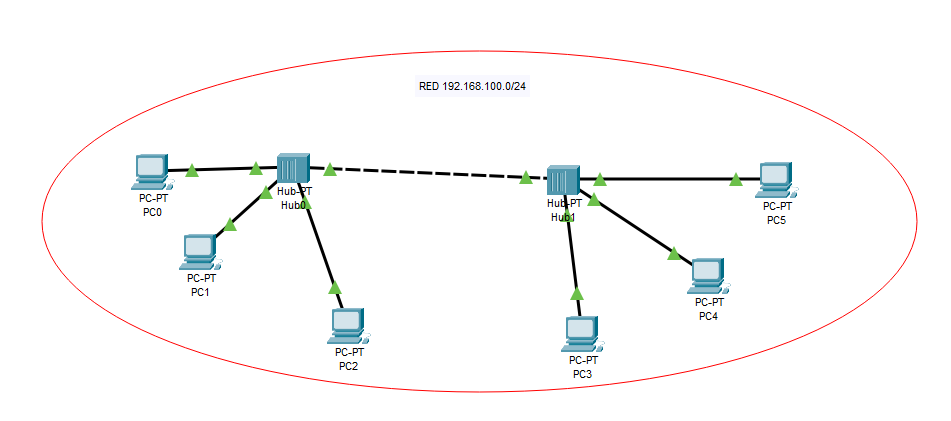
\includegraphics[scale=0.5]{Act/1.PNG}
    \begin{enumerate}
        \item Copper straight-through: es un tipo de cable de cobre de par trenzado para red de área local ( LAN ) uso para el que los conectores RJ-45 en cada extremo tienen el mismo pinout (es decir , la disposición de los conductores ). Es idéntico al cruce del cable , excepto que en este último los alambres en el cable se cruzan de manera que el recibir pernos de la señal en el conector en un extremo están conectados a los pernos de la señal de transmisión en el conector en el otro extremo
        \item Copper cross-over: Un cable cruzado conecta dos dispositivos del mismo tipo , por ejemplo DTE - DTE o DCE - DCE , por lo general conectados de forma asimétrica ( DTE - DCE ) , por un cable modificado denomina reticulación . Tal distinción de los dispositivos fue introducido por IBM .
    \end{enumerate}
    \item Desde consola haga ping de PC0 a PC2, observe los resultados e identifique los protocolos usados
    
    \begin{enumerate}
        \item Ping PC0->PC2\\
        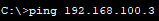
\includegraphics[scale=1]{Act/2_1.PNG}    
        \item Resultados\\
        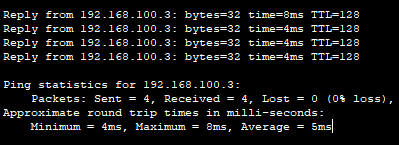
\includegraphics[scale=1]{Act/2_2.PNG}
        \item Protocolos\\
        \begin{itemize}
            \item ICMP:El Protocolo de Mensajes de Control y Error de Internet, ICMP
            \item ARP:El Protocolo de resolución de direcciones
        \end{itemize}
    \end{enumerate}
    \item Desde consola haga ping de PC0 a PC5, observe los resultados, cual es la diferencia, identifique los protocolos usados
    \begin{enumerate}
        \item Ping PC0->PC5\\
        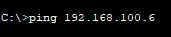
\includegraphics[scale=1]{Act/3_1.PNG}
        \item Resultados\\
        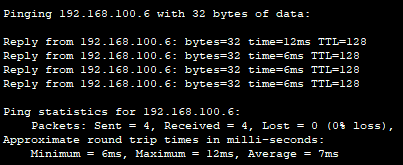
\includegraphics[scale=1]{Act/3_2.PNG}
        \item Diferencia\\
        La diferencia radica en que el PC5 se encuentra en que el PC0 y el PC5 estan conectados en diferentes hubs lo cual hace que para lograr enviar el ping  al PC5 tendra que pasar por dos hubs lo que hara que se demore mas tiempo del habitual como se muestra en los resultados.
        \item Protocolos\\
        \begin{enumerate}
            \item ICMP:El Protocolo de Mensajes de Control y Error de Internet, ICMP
            \item ARP:El Protocolo de resolución de direcciones
        \end{enumerate}
    \end{enumerate}
    \item Agregue PC6 usando un hub adicional, haga un ping de consola de PC4 a PC5, luego a PC0 y finalmente a PC6, ¿cuál es la diferencia?,¿porque?\\
    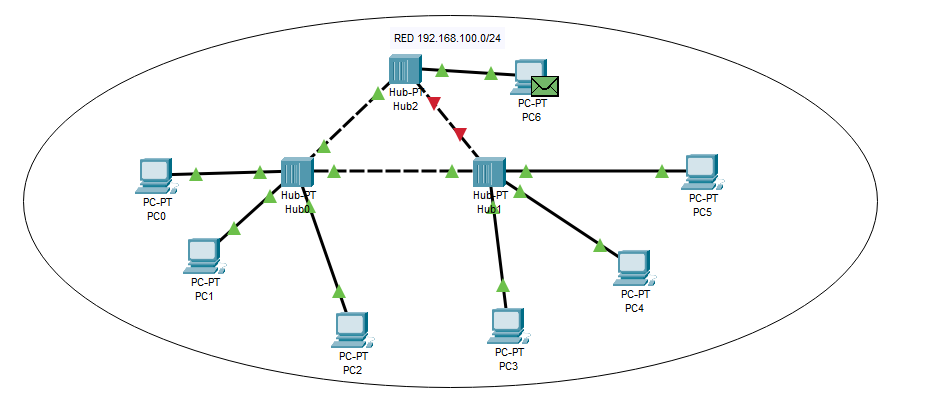
\includegraphics[scale=0.5]{Act/4.PNG}
    \begin{enumerate}
        \item ping PC4->PC5\\
        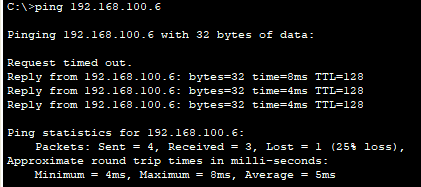
\includegraphics[scale=1]{Act/4_1.PNG}
        \item ping PC0->PC6\\
        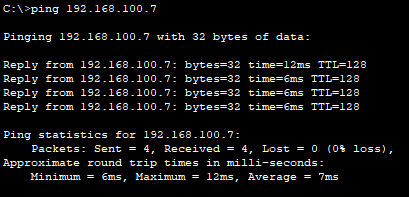
\includegraphics[scale=1]{Act/4_2.PNG}
        \item Diferencia\\
        El tiempo de demora PC0->PC6 es mayor que el de PC4->PC5 casi el doble ya que este esta en otro hub.\\
        En algunos casos se da perdida en en los envios como se ve en los resultados.
    \end{enumerate}
    \item ¿Encuentra alguna deficiencia en la configuración anterior?, explique observando la simulación del paso 4.4
    \begin{itemize}
        \item Al ser hub envia mucha data entre los hubs por lo cual si se envia en ese momento mas data se perdera informacion en ciertos casos.
    \end{itemize}
    \item Incorpore el bridge tal como se muestra en la figura y repita 4.1 a 4.3 ¿Qué diferencia encuentra en el comportamiento de la red? ¿en que difiere el comportamiento al agregar un bridge en lugar del cableado directo? Describa brevemente la función del bridge, indique además si hay alguna diferencia en los protocolos usados
    \begin{enumerate}
        \item 4.1:\\
        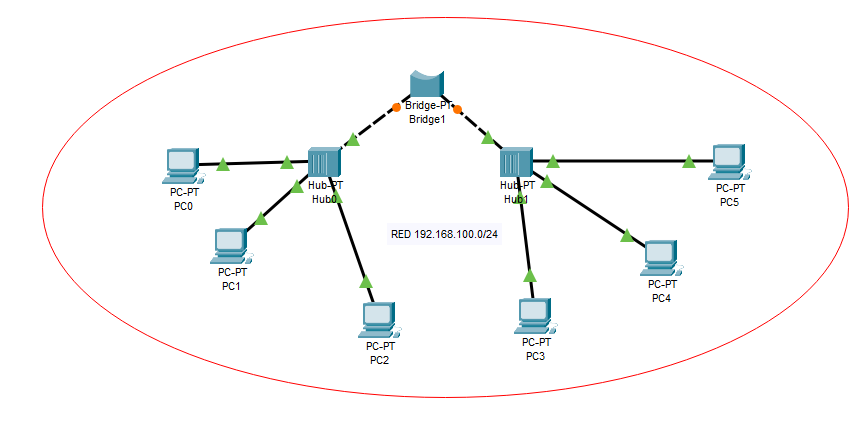
\includegraphics[scale=0.5]{Act/6.PNG}
        \item 4.2: ping PC0->PC2\\
        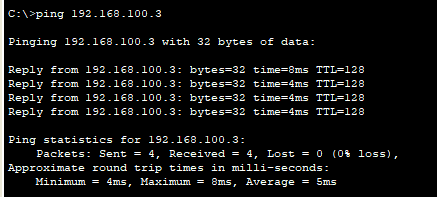
\includegraphics[scale=0.5]{Act/6_1.PNG}
        \begin{itemize}
            \item Protocolos
            \begin{itemize}
                \item ICMP:El Protocolo de Mensajes de Control y Error de Internet, ICMP
                \item ARP:El Protocolo de resolución de direcciones
                \item STP
            \end{itemize}
        \end{itemize}
        
        \item 4.3: ping PC0->PC5\\
        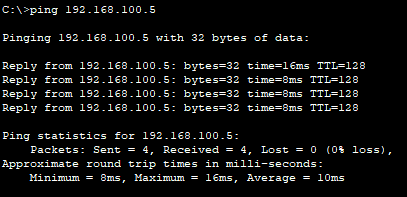
\includegraphics[scale=0.5]{Act/6_2.PNG}
        \begin{itemize}
            \item Protocolos
            \begin{itemize}
                \item ICMP:El Protocolo de Mensajes de Control y Error de Internet, ICMP
                \item ARP:El Protocolo de resolución de direcciones
                \item STP
            \end{itemize}
        \end{itemize}
        \item Diferencias\\
        La diferencia es el tipo de conexion que llevan lo hubs, en la primera estan conectados directamente y el segunda estan conectados por un bridge la que actua como switch evitando envio de data no necesaria.
        \item Descripción\\
        El bridge actua igual que un switch siendo capaz de conectar segmentos de red formando una sola subred (permite conexión entre equipos sin necesidad de routers)
    \end{enumerate}
    \item Reemplace los hubs por switchs tal como se muestra y repita de 4.1 a 4.6, observando en modo simulación ¿qué diferencias encuentra? ¿Porque?
    \item Incorpore dos computadoras a través de un switch adicional, espere la autoconfiguración. Haciendo un ping desde consola observe las diferencias al conectar PC0 con PC2, luego con PC3 y finalmente con PC7. Simule y luego explique los resultados, el funcionamiento de switchs y bridge, indique los protocolos usados
    \item Implemente el siguiente subneteo y haciendo ping desde consola verifique que la interconectividad funcione correctamente. Resuma en una tabla la dirección IP, la máscara y a que red y subred pertenece cada PC, indique para cada una el rango de direcciones IP, el subfijo, el número de hosts disponibles, la dirección de red y la dirección de difusión (tome como referencia las tablas de conectividad de la práctica anterior)
    \item 
\end{enumerate}

\newpage


%\begin{thebibliography}{9}

%\bibitem{algebra} Quispe, S.(2013).Percepción ambiental del proceso de desertificación en el Perú.\textit {Investigaciones sociales,17(30),47-57.}

%\end{thebibliography}

\end{document}